\documentclass{amsbook}
\usepackage[utf8]{inputenc}

%\documentclass[a4paper,11pt]{amsart}

\usepackage{graphics}

%\usepackage{arxiv}
%\usepackage{enseign}
%\usepackage[utf8]{inputenc} % allow utf-8 input
\usepackage[T1]{fontenc}    % use 8-bit T1 fonts

\usepackage{amsthm}
\usepackage{amsbsy,amsmath,amssymb,amscd,amsfonts}
%\usepackage[pagebackref=true]{hyperref}
\usepackage{hyperref}
\usepackage{url}            % simple URL typesetting
\usepackage{booktabs}       % professional-quality tables
\usepackage{nicefrac}       % compact symbols for 1/2, etc.
\usepackage{microtype}      % microtypography

\usepackage{graphicx,float,latexsym,color}
%\usepackage{refcheck}
%\usepackage{mathspec}
\usepackage[font={small,it}]{caption}
\usepackage{subcaption}
%\let\proof\relax
%\let\endproof\relax

\usepackage{makecell}
\renewcommand{\arraystretch}{1.2}

\usepackage[dvipsnames]{xcolor}

\newtheorem{theorem}{Theorem}
\newtheorem{observation}{Observation}
\newtheorem{proposition}{Proposition}
%\newtheorem{remark}{Remark}

\newtheorem{corollary}{Corollary}
%\newtheorem{definition}{Definition}
\newtheorem{lemma}{Lemma}
\newtheorem{question}{Question}

\theoremstyle{definition}
\newtheorem{definition}{Definition}
\newtheorem{remark}{Remark}
% suggestion of reviewer
%\theoremstyle{definition}
%\newtheorem{definition}{Definition}
%\newtheorem{remark}{Remark}

\hypersetup{
    %bookmarks=true,         % show bookmarks bar?
    %unicode=true,          % non-Latin characters in Acrobat’s bookmarks
    pdftoolbar=true,        % show Acrobat’s toolbar?
    pdfmenubar=true,        % show Acrobat’s menu?
    pdffitwindow=false,     % window fit to page when opened
    pdfstartview={FitH},    % fits the width of 
    colorlinks=true,       % false: boxed links; true: colored links
    linkcolor=OliveGreen,          % color of internal links (change box color with linkbordercolor)
    citecolor=blue,        % color of links to bibliography
    filecolor=black,      % color of file links
    urlcolor=red           % color of external links
}

\usepackage{lineno}
\def\linenumberfont{\normalfont\small\sffamily}
%a4: 210 x 297
%\textwidth=125mm
%\textheight=195mm
\arraycolsep=2pt
\captionsetup{width=120mm}

\title[An Exp. Promenade around the Ell. Billiard]{An Experimental Promenade\\Around the Elliptic Billiard}
% authors in alpha order
\author[R. Garcia]{Ronaldo Garcia}
\author[D. Reznik]{Dan Reznik} 


\date{January, 2021}

\begin{document}

\maketitle

\chapter{Introduction}
\label{sec:intro}
Poncelet N-periodics are families of N-gons inscribed in a first conic while simultaneously circumscribing a second conic \cite{dragovic11}. We continue our study of loci and invariants of Poncelet 3-periodics (see related work below). Previously we focused on families interscribed between concentric, axis-aligned ellipse pairs. Here we expand the analysis to a generic pair of nested ellipses and explore (i) the power of the center with respect to well-known circles, and (ii) loci of triangle centers under various ellipse arrangements, see Figure~\ref{fig:n3-general-pos}. Recall triangle centers are points in the plane of a triangle (e.g, incenter, circumcenter, etc.) whose trilinear coordinates obey certain conditions \cite{kimberling1993_rocky}.

\begin{figure}
    \centering
    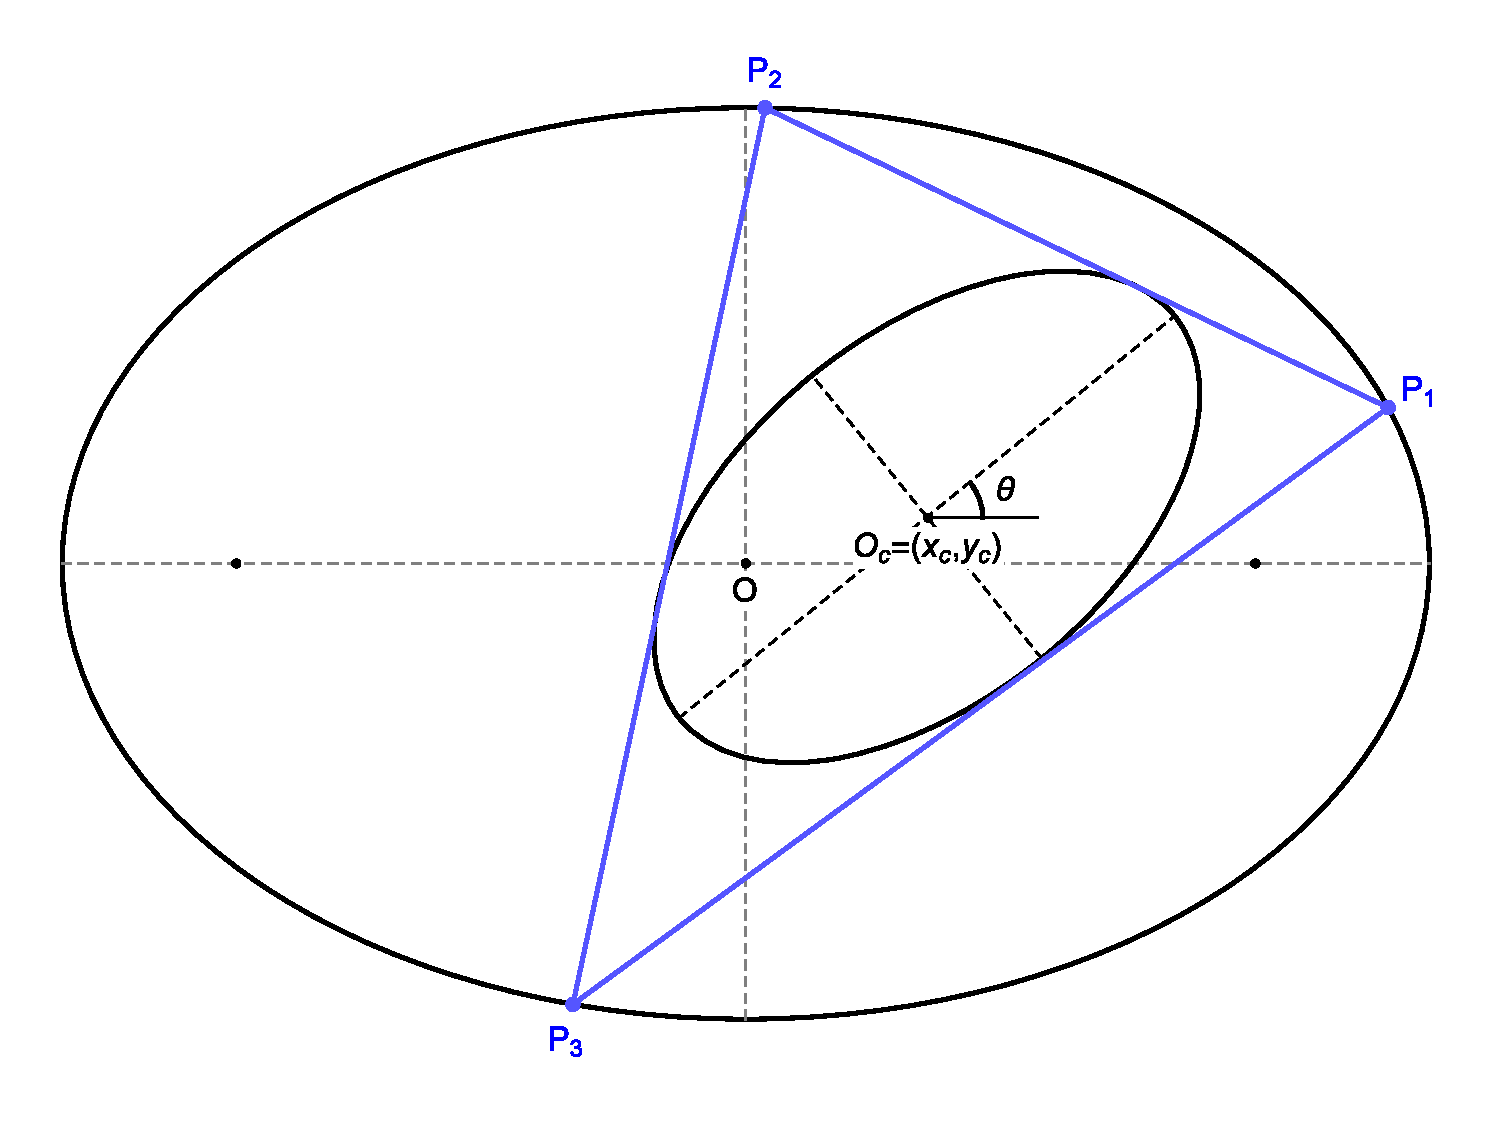
\includegraphics[width=.6\textwidth]{pics/0070_n3_nonconcentric.eps}
    \caption{A pair of ellipses in general position which admits a Poncelet 3-periodic family (blue). Let the outer one be centered at the origin $O$. Their major axes are tilted by $\theta$, and their centers displaced by $O_c=(x_c,y_c)$. \href{https://youtu.be/bjHpXVyXXVc}{Video}}
    \label{fig:n3-general-pos}
\end{figure}

\subsection*{Main Results}

\begin{itemize}
  \item Section~\ref{sec:axis-aligned}: We first show that over 3-periodics in several concentric, axis-aligned pairs -- confocal, homothetic, with incircle, with circumcircle, and excentral -- the power of the center with respect to either the circumcircle or Euler's circle is invariant. Using analytic geometry (with trilinear coordinates), we derive explicit formulas for said powers for each family.
  \item Section~\ref{sec:concentric-tilted}: using CAS-based manipulation, we generalize this by proving that the power of the center with respect to both Euler's circle and the circumcircle is invariant for 3-periodics for any generic concentric pair (aligned or not), Theorem~\ref{thm:power-concentric-unaligned}.
    \item Section~\ref{sec:nonconcentric-circumcircle}: We then consider 3-periodics in the non-concentric pair with circumcircle. Using  a special parametrization based on Blaschke products \cite{daepp-2019}, we show that loci of triangle centers which are fixed affine combinations of the barycenter and circumcenter are circles, whose centers are collinear along a line passing through the stationary circumcenter.
    \item Section~\ref{sec:nonconcentric-tilted} For the generic case of 3-periodics in the non-concentric, non-axis-aligned ellipse pair, we show that triangle centers which are fixed linear combinations of barycenter and circumcenter will trace out elliptic loci, Theorem~\ref{thm:ellipse-locus}. These include such centers as the orthocenter, the center of the Euler circle, the de Longchamps point, etc.; see Observation~\ref{obs:affine-euler-line}.
\end{itemize}

In Section~\ref{sec:open-questions} we conclude with a few experimental conjectures. Appendix~\ref{app:symbols} contains a list of symbols used herein.

\subsection*{Related Work}

In \cite{odehnal2011-poristic}, the loci of many triangle centers over the poristic family (fixed circumcenter and incenter) are shown to be either stationary, circular, or elliptic. In \cite{sergei2016-com}, the loci of vertex and area centroids are proved to be ellipses over a generic Poncelet family. The circumcenter of mass (which is simply the circumcenter for Poncelet 3-periodics) is shown to be an ellipse in \cite{sergei2014-circumcenter-of-mass}.
 
 Properties of 3-periodics in the confocal pair (elliptic billiard) were studied in \cite{reznik2020-intelligencer,garcia2020-new-properties}. A few results and their subsequent proofs include: the elliptic locus of the incenter \cite{olga14,garcia2019-incenter}, circumcenter \cite{garcia2019-incenter,corentin19}, invariant sum of cosines  \cite{akopyan2020-invariants,bialy2020-invariants}, and invariant ratio of outer-to-orbit polygon areas  \cite{caliz2020-area-product}. 
 
In \cite{garcia2020-ellipses} it was shown that over confocal 3-periodics, 29 triangle centers (out of the first 100 in \cite{etc}) trace out ellipses. Explicit expressions are given for the semi-axes of each locus. In subsequent works, we studied the relationship between (i) poristic triangles and the confocal family (poristic) \cite{garcia2020-similarity-I}, and (ii) the homothetic family and the Brocard porism \cite{reznik2020-similarityII}, showing that said pairs are images of each other under a variable similarity transform. In \cite{garcia2020-family-ties} we compare several loci and invariants across several concentric, axis-aligned pairs, grouping them into clusters.


 


\chapter{Elliptic Billiard Preliminaries}
\label{sec:preliminaries}


%\begin{figure}
%    \centering
%    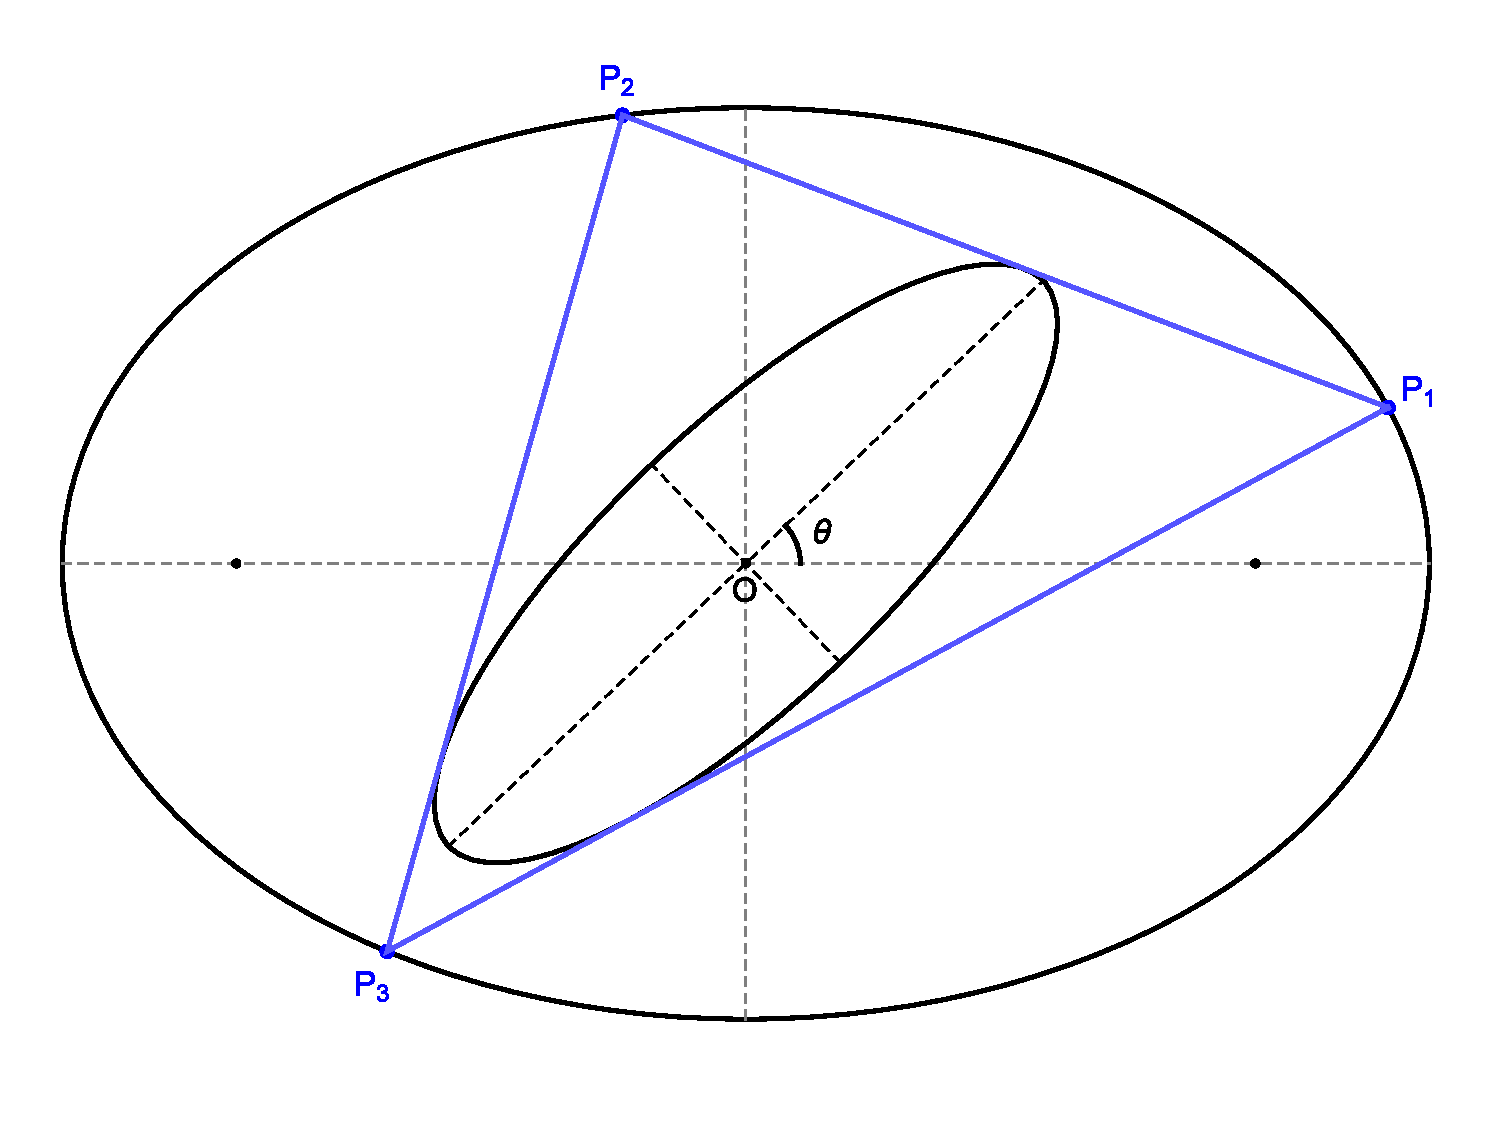
\includegraphics[width=.7\textwidth]{pics/0020_n3_tilted.eps}
%    \caption{A concentric, unaligned pair of ellipses which admits a 3-periodic family (blue). Their major axes are tilted by $\theta$.}
%    \label{fig:n3-tilted}
%\end{figure}

Consider two nested ellipses $\E$ and $\E_c$ with semi-axes $(a,b)$ and $(a_c,b_c)$: $\E$ is centered at the origin $O$ and $\E_c$ at $O_c=(x_c,y_c)$. Let $\theta$ denote the angle between their major axes; see Figure~\ref{fig:n3-general-pos}. If $O_c=0$ we call the pair ``concentric''. If $\theta=0$ we call it ``axis-aligned''. Additionally, let $c^2={a^2-b^2}$ and $c_c^2={a_c^2-b_c^2}$ denote their half focal distances. Note these are the squares of half the focal distance.

\begin{definition}
The power $\P_X$ of a point $X$ with respect to a circle centered on $C$ and of radius $R$ is given by \cite[Circle Power]{mw}:

\[ \P_X(C,R) = |X-C|^2-R^2 \]
\end{definition}

Recall the circumcircle passes through triangle vertices. Using Kimberling's notation for triangle centers \cite{etc}, let $X_3$ and $R$ denote its center and radius; these are known as circumcenter and circumradius. Also recall Euler's (or Feuerbach's, or the 9-point) circle: it passes through the sides' midpoints. Its radius is half the circumradius \cite[Nine-point circle]{mw}. Let $X_5$ denote its center. The following shorthands will be used for the power of a point $O$ wrt to either circumcircle or Euler's circle:

\[ \P_3 = \P_{O}(X_3,R),\;\;\;\P_5 = \P_{O}(X_5,R/2) \]


\chapter{The Locus of the Incenter}
\label{sec:loci}
\input{020_incenter}

\chapter{The Invariant Sum of Cosines}
\label{sec:cosines}
\input{030_cosines}

\chapter{The Invariant Inversive Perimeter}
\label{sec:inv-perimeter}
\input{040_inversive_perimeter}

\chapter{Poncelet with Circumcircle and Blaschke Products}
\label{sec:circumcircle}
\input{050_poncelet_circumcircle}

\chapter{Experimental Techniques}
\label{sec:experimental}
\section{Main Result}

History. How to obtain vertices of N-periodic. Cayley determinants. Birkhoff counting of self-intersected.

\begin{theorem}
For $N=5$, given the semi-axes $(a,b)$ of the elliptic billiard, those of the caustic are a root of the following sextic equation:

\[ ... \]
\end{theorem}

\section{Vertices via Numerical Optimization}

\section{Elliptic N-Periodics App}





\chapter{Conclusion}
\label{sec:conclusion}
Animations illustrating some of the above phenomena are listed on Table~\ref{tab:playlist}.

\begin{table}
\small
\begin{tabular}{|c|l|l|}
\hline
id & Title & \textbf{youtu.be/<.>}\\
\hline
01 & {Cayley-Poncelet Phenomena I: Basics} &
\href{https://youtu.be/virCpDtEvJU}{\texttt{virCpDtEvJU}}\\
02 & {Cayley-Poncelet Phenomena II: Intermediate} &
\href{https://youtu.be/4xsm\_hQU-dE}{\texttt{4xsm\_hQU-dE}}\\
\hline
\end{tabular}
\caption{Videos of some focus-inversive phenomena. The last column is clickable and provides the YouTube code.}
\label{tab:playlist}
\end{table}

The following questions are posed to the reader:



\noindent We would like to thank A. Akopyan for valuable insights. The third author is fellow of CNPq and coordinator of Project PRONEX/ CNPq/ FAPEG 2017 10 26 7000 508.

\appendix

\section{Focal Properties of Conics}
\label{app:focal}
\input{130_focal_properties}

\section{Other Types of Billiards}
\label{app:other-billiards}
\input{140_other_billiards}

\section{Table of Symbols}
\label{app:symbols}
\begin{table}[H]
\small
\begin{tabular}{|c|l|}
\hline
symbol & meaning \\
\hline
$\E,\E_c$ & outer and inner ellipses \\
$O,O_c$ & centers of $\E$,$\E_c$\\
$a,b,a_c,b_c$ & outer and inner ellipse semi-axes' lengths \\
$c,c_c$ & half-focal length of $\E,\E_c$ \\ 
 $O_c=(x_c,y_c)$\\
$\theta$ & major semi-axis tilt $\E_c$ wrt $\E$ \\
$P_i,s_i$ & 3-periodic vertices and sidelengths \\
$r,R$ & 3-periodic inradius and circumradius \\
$a_i,b_i$ & semiaxes of the locus of $X_i$ \\
$r_i$ & radius of the locus of $X_i$ (if $a_i=b_i$) \\
\hline
$\C_3,\C_5$ & circum- and Euler's circle \\
$\C_2,\C_{381}$ & Steiner orthoptic and orthocentroidal circle \\
$\C_4,\C_{26}$ & polar and tangential circle \\
$\P_i$ & power of center $O$ wrt $\C_i$ \\
\hline
$X_1,X_2,X_3$ & Incenter, Barycenter, Circumcenter \\
$X_4,X_5,X_6$ & Orthocenter, Euler center, Symmedian point \\
$X_9,X_{20}$ & Mittenpunkt, de Longchamps point\\
\hline
\end{tabular}
\caption{Symbols used in the article.}
\label{tab:symbols}
\end{table}

\section{Original Proposal}

\begin{figure}
    \centering
    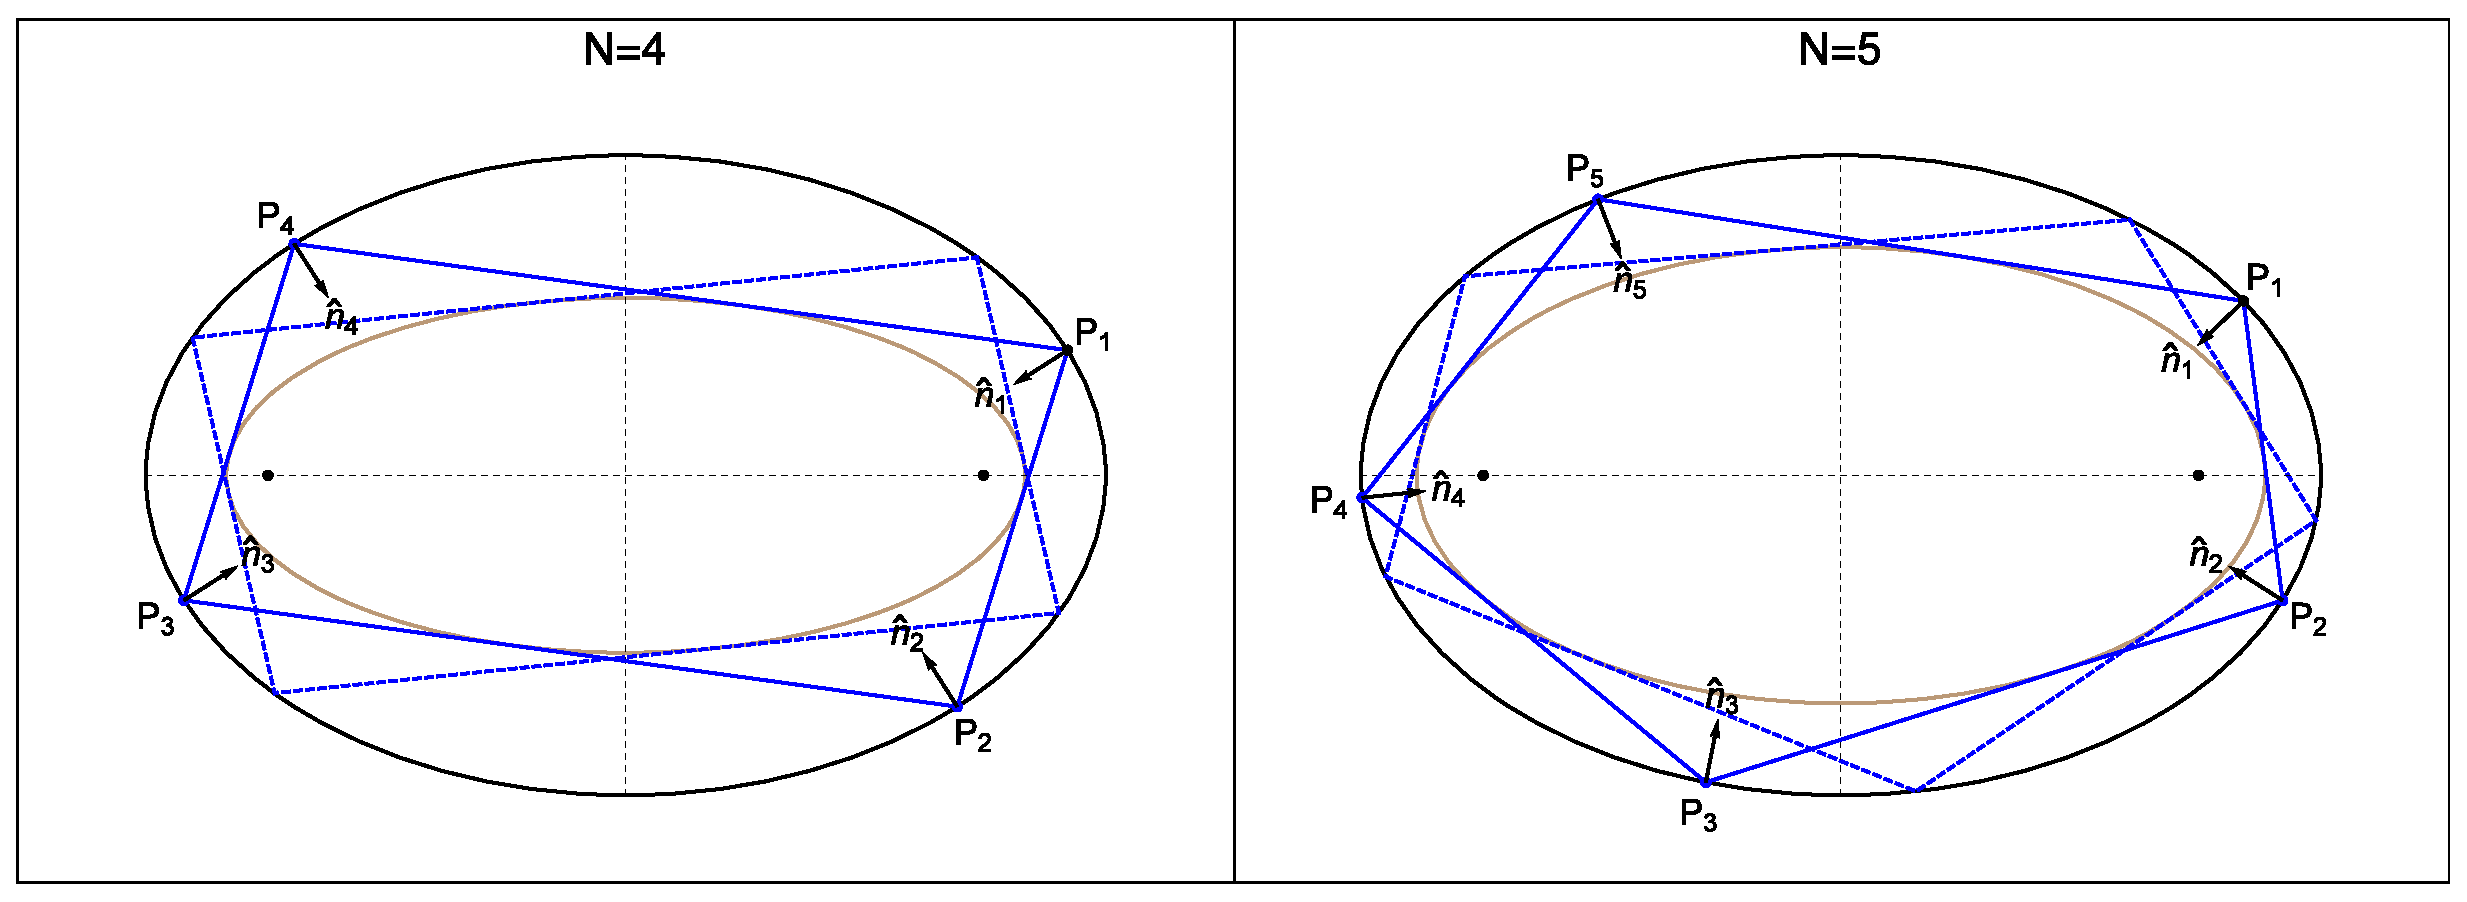
\includegraphics[scale=0.35]{pics_proposal/0000_n4n5.eps}
    \caption{Bilhar Elíptico e (4,5)-órbitas periódicas (azul) . Em todo vértice o vetor normal $\hat{n}_i$ bissecta os segmentos   de órbitas bilhares  $P_{i-1} P_{i}$ e $P_i P_{i+1}$ que são tangentes à cáustica (marrom). Uma segunda órbita também é mostrada (azul pontilhado). Note que o perímetro é conservado sobre toda a família de N-periódicas.   \href{https://youtu.be/Y3q35DObfZU}{Video}}
    \label{fig:n4n5}
\end{figure}
 \newpage
\begin{enumerate}
    \item \textbf{Nível}: Introdutório.
    \item \textbf{Duração}: 5 aulas de 45 minutos.
    \item \textbf{Descrição detalhada}: 
    \begin{itemize}
        \item \textbf{Objetivos}: Introdução à geometria dos bilhares elípticos \cite{darboux1917,lebesgue1942,rozikov2018,sergei91}, tema de grande influência na matemática dos últimos 200 anos. Divulgar novos invariantes ali manifestados, o método experimental de descoberta, e esboçar algumas provas.
        \item \textbf{Público-Alvo}: aluno(a)s de graduação ou pós, professores, ou quaisquer interessado(a)s em conhecer novas e belas propriedades do bilhar elíptico encontradas experimentalmente.
        \item \textbf{Conteúdo}: Geometria do bilhar elíptico, porisma de Poncelet e condições de Cayley \cite{dragovic11}, loci de centros triangulares \cite{etc} sobre a fam\'ilia de 3-periódicas, órbitas auto-intersectadas, polígonos inversivos, outras famílias Ponceletianas. Exemplificar alguns fenômenos por vídeos \cite{reznik2020-youtube} e/ou ferramenta interativa \cite{reznik2020-app}.
        \item \textbf{Monitoria}: co-autores e/ou alunos de iniciação científica farão revezamento.
        \end{itemize}
        \item \textbf{Distribuição de capítulos}:
        \begin{itemize}
            \item  Capítulo 1: Propriedades focais das cônicas \cite{akopyan2007-conics,berger1987,darboux1917,lebesgue1942}. Família confocal de cônicas. Relações entre elipses e triângulos (inscritos e circunscritos). 
            Introdução ao bilhar elíptico e ao porisma de Poncelet.  Condições de Cayley.
             Exercícios e projetos.
            
            \item Capítulo 2:
             Centros triangulares (incentro, baricentro, circuncentro, ortocentro, mittenpunkt etc). Coordenadas trilineares e baricêntricas no plano. Propriedades básicas de alguns  centros triangulares  \cite{ coxeter67,   kimberling98} e triângulos derivados (pedal, tangente, excentral etc).
            Loci e Invariantes Básicas: Loci elípticos de centros triangulares, soma de cossenos, razão de áreas, potência de um ponto em relação a um círculo.  Método experimental e algebro-computacional \cite{  garcia2019-incenter, garcia2020-ellipses, garcia2020-new-properties}.
            Exercícios e projetos.
            %Sketch das provas já publicadas. \cite{akopyan2020-invariants,bialy2020-invariants,caliz2020-area-product}.
            
            \item Capítulo 3: N-periodicas auto-intersectadas, condições de Birkhoff \cite{birkhoff66}. \textit{Tour } de N-periódicas auto-intersectadas. Exercícios e projetos.
            
            \item Capítulo 4: Inversão com respeito a um círculo. O talentoso polígono foco-inversivo, seus invariantes e propriedades. Exceções em invariantes. Exercícios e projetos.
            %Conexão com a transformação de Moebius.
            \item Capítulo 5: Alguns invariantes em outras famílias Ponceletianas, e.g., homotética, porística, com incírculo, circumcírculo  etc. Exercícios e projetos.
            
               \item Capítulo 6:  Tópicos de bilhares em curvas convexas e polígonos. Uma conexão rápida com vários outros ramos da matemática, contextualizando os problemas em aberto. Resenha de problemas de investigação no contexto de bilhares.
               
        \end{itemize}
        \item Pré-requisitos: conhecimentos básicos de Construções Geométricas,  Geometria Analítica, Álgebra Linear e Cálculo Diferencial.
        
        \item Número de páginas: Uma estimativa preliminar é de 120 páginas com muitas figuras ilustrando as propriedades geométricas observadas em experimentos computacionais no  bilhar elíptico e links para vídeos no youtube.
        
        \item Outras informações: a boa recepção da nossa palestra de divulgação  ``Aventuras com Triângulos e Bilhares'' ministrada no 32$^{\underline{o}}$  CBM do IMPA (2019) \cite{reznik2019-impa-talk,reznik2019-impa-article} além de nossas publicações em 2020  \cite{reznik2020-intelligencer,garcia2020-ellipses,garcia2020-new-properties,reznik2020-ballet,reznik2021-circum,reznik2021-fifty-invariants,garcia2020-similarity-I,garcia2020-steiner,reznik2020-similarityII,garcia2020-self-intersected,reznik2020-n3-focus-inversive}, nos motivou em propor esse curso com novos resultados e mais detalhes das técnicas utilizadas.
        \vskip .5cm
       Anexo segue artigo aceito para publicação na revista Amer. Math. Monthly ilustrando alguns resultados obtidos pelos proponentes. Também anexamos o artigo publicado na revista Math. Intelligencer.
        
\end{enumerate}







\bibliographystyle{maa}
\bibliography{references,authors_rgk_v3}

\end{document}
